\documentclass[sigconf, review=false]{acmart}
\usepackage[english]{babel}
\usepackage{graphicx}
\graphicspath{ {./images/} }
\author{Jeroen-Niclas Trzaska}
\title{DB proseminar - Isolation Levels}
\acmDOI{}
\acmISBN{}
\acmConference{Proseminar}{WS2020/2021}{}
\settopmatter{printacmref=false}

\affiliation{%
   \institution{TU Dresden}
   \city{Dresden}
   \state{Saxony}
   \country{Germany}}
\email{jeroen-niclas.trzaska@mailbox.tu-dresden.de}

\citestyle{acmauthoryear}
\begin{document}

\begin{abstract}
    This paper is going to look at the strengthened ANSI SQL phenomena definition propositions
    by \cite{Adya_Liskov_O_Neil_2000} as well as the corresponding isolation levels,
    comparing them in terms of strength. It will also take a quick look at non lock based implementations
    and the problems the ANSI SQL standard has in regards to such implementations as shown in \cite{Berenson_Bernstein_Gray_Melton_O_Neil_O_Neil_1995}.
\end{abstract}
\maketitle

\section{Motivation}
The motivation behind these analyses of the ANSI SQL standard is to better define and examine the
behavior of different database implementation approaches when presented with multi-item dependencies.
This is important as the ANSI standard was created when locking implementations where the norm and thus multi version systems were not
taken into consideration when creating it, leading to unexpected behavior not in line with ANSI SQL.
These issues include but are not limited to dependency constrains between two items in a database. \\
For example assume that Alice has two accounts at a bank, the accounts can be overdrawn as long as the sum is greater or equal to 0.
She has 20€ on each of the accounts. Now she withdraws 30€ from account A and another 20€ form account B.
Looking at each of the transactions out of context, we can see that the constraint $A+B \geq 0$ is met.
But when executed simultaneously the resulting sum of $A$ and $B$ can still be negative. To achieve this outcome
Alice asks Bob to help her.
\begin{example}
    Alice reads 20€ to be in both accounts and Bob does the same. Alice then
    withdraws 30€ from account A and writes -10€ into it and commits, the constrain,
    $A+B \geq 0$, is still met.
    Bob then withdraws 20€ from account and, as his transaction had read both accounts to have
    20€, he writes 0€  to B. Both transactions commit and the committed data in the database now violates the constrain $A+B \geq 0$.
\end{example}
The following figure visualizes the relation between the phenomena and isolation levels that will be defined
at a later point in this paper. Starting with the weakest level of isolation (Degree 0) each arrow denotes the phenomenon to be prohibited
by the next isolation level.
\begin{figure}[H]
    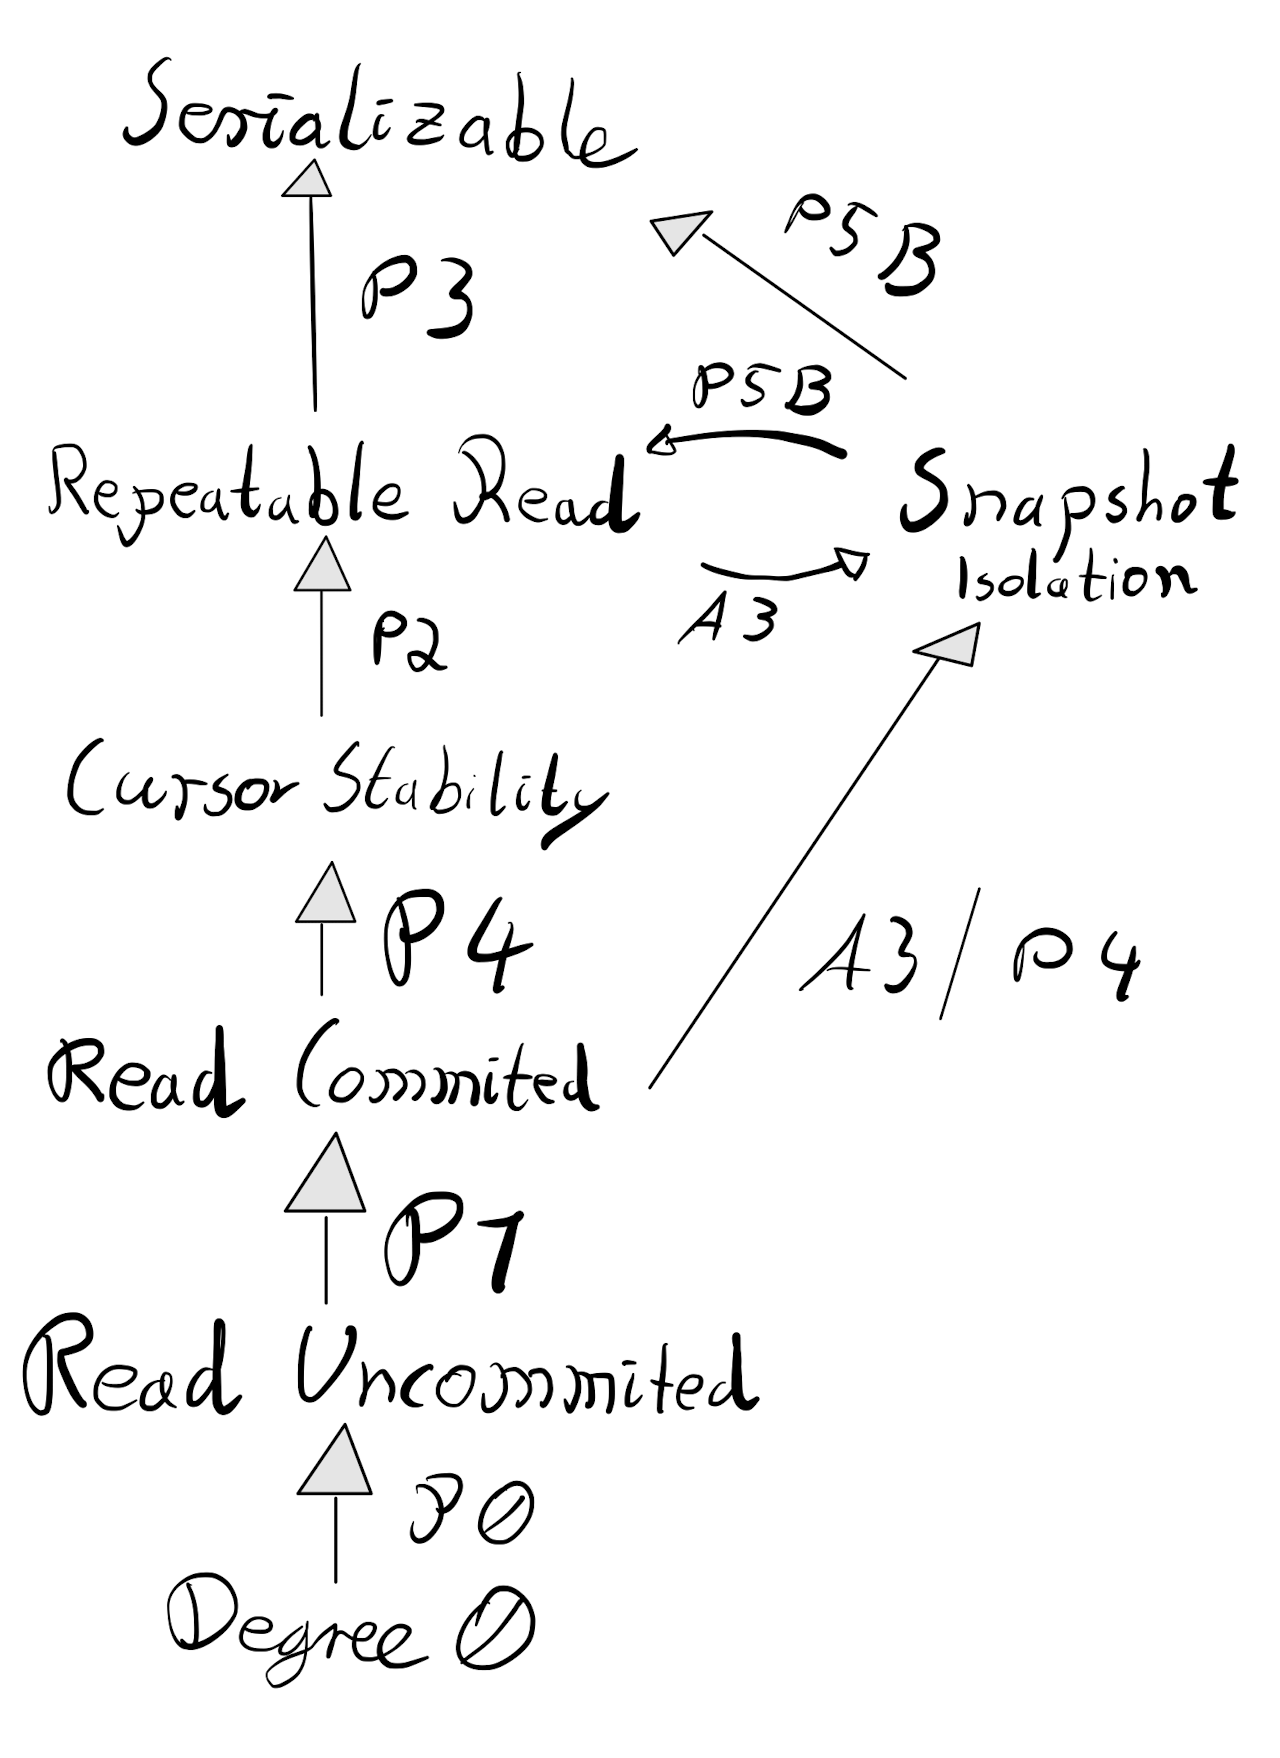
\includegraphics[width=8.5cm, height=9.5cm]{iso_lvl_dia.png}
    \caption{isolation level diagram}
    \Description{isolation level diagram}
\end{figure}
\section{Phenomena Definitions}
We are now going to introduce the strengthened ANSI phenomena definitions as described in \cite{Adya_Liskov_O_Neil_2000} which
are based on the broad interpretation of the ANSI SQL standard. These definitions are inherently stronger then their ANSI counter part,
as they rule out more phenomena as defined in the following paragraphs. This is due to the fact that the ANSI standard
was created with locking implementations in mind. Leading to definitions that would allow phenomena to appear in the database's history when using non lock based systems
while lock based systems using the same interpretation would not allow them.

\subsection{P0 - Dirty write}
An example for the above mentioned problem with the strength of ANSI SQL is that while a locking implementation of \emph{read uncommitted}
prevents the following phenomenon, a non locking system would not do so (see s
section 2.2 of \cite{Adya_Liskov_O_Neil_2000}).
We start by defining the first phenomena, which describes two consecutive writes by two different
transactions leading to an undefined value for x in case the first transaction aborts.

\begin{example}
    Alice deposits 10€ into a bank account x.
    Bob than deposits a further 20€ into the same account.
    To do so he reads the value of x and then adds 20€ and writes it back to the account x.
    Alice than performs a rollback on her transaction.
    Thus the amount of money in account x is unclear.
\end{example}

\begin{figure}[h]
    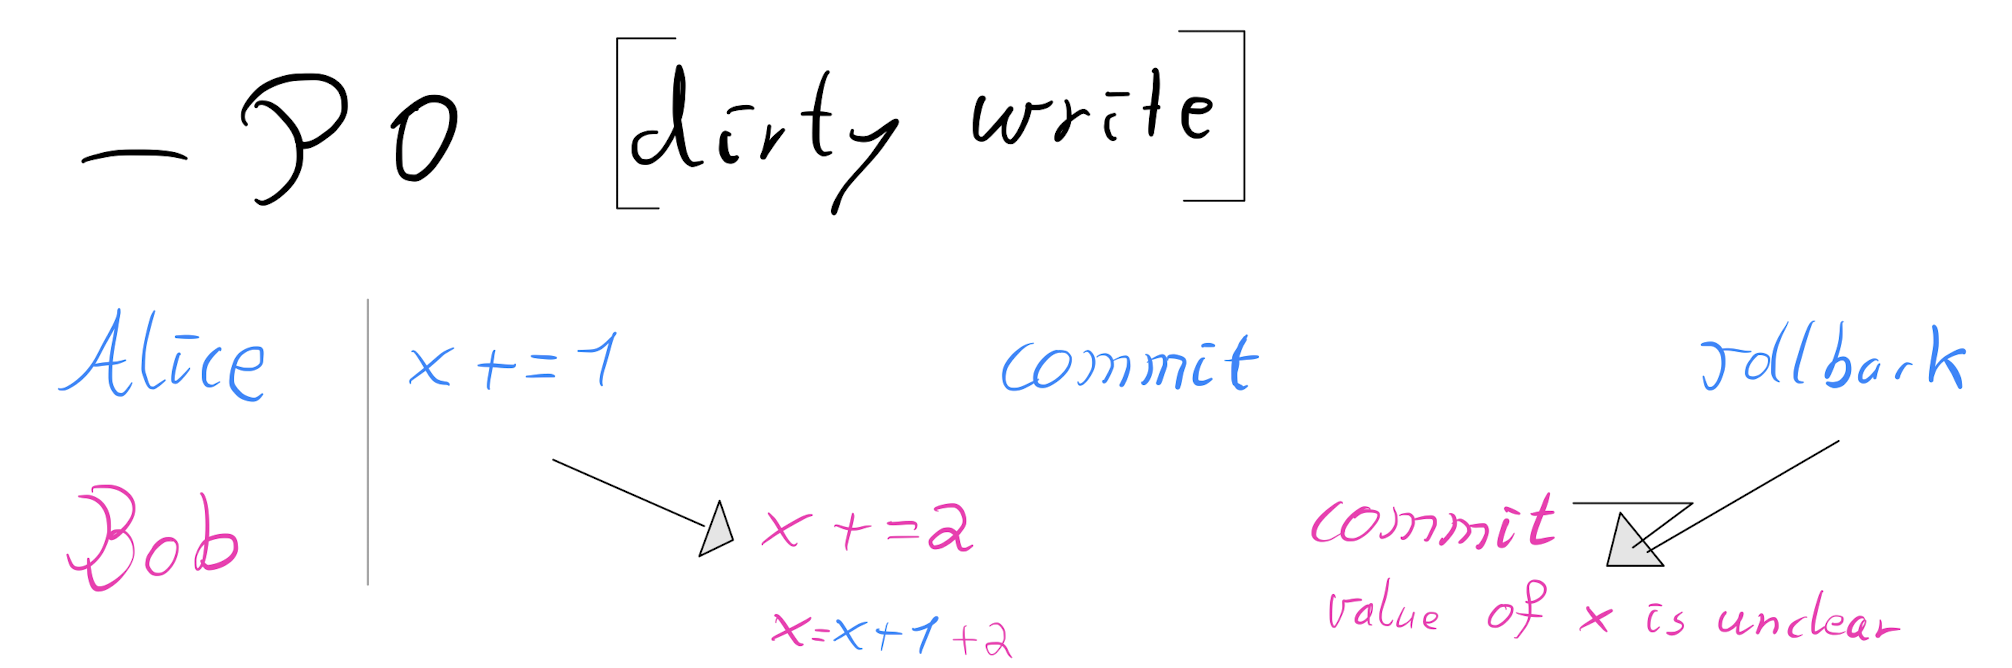
\includegraphics[width=8.5cm]{P0}
    \caption{History for P0}
    \Description{P0}
\end{figure}

\subsection{P1 - Dirty read}
For the second phenomenon we are going to look at reading inconsistent data from the database.
This can be a problem when retrieving information while another transaction
that writes data is being executed. An issue that can arise when this phenomenon is not prohibited,
is that the given transaction reading the inconsistent data will continue to work with this
incorrect data and writing wrong data back to the database, corrupting it in the process.

\begin{figure}[h]
    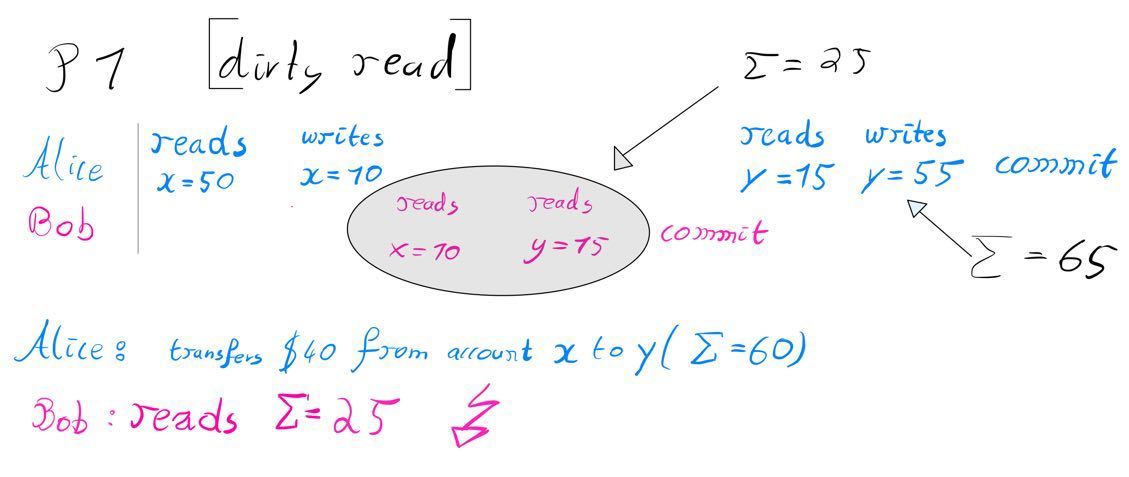
\includegraphics[width=8.5cm]{P1}
    \caption{History for P1}
    \Description{P1}
\end{figure}

\begin{example}
    Alice transfers 40€ form account x to account y.
    To do so she reads the value of x subtracts the 40€ writing 10€ to value of x.
    Afterwards, Bob reads the value of x (10€) and y (15€) resulting in a sum of 25€
    Alice then reads the value of y (15€) and then adds the 40€ to it resulting in a sum of 55€ for y
    and a total of 65€.
\end{example}

\subsection{P2 - Fuzzy read}
The next phenomenon is similar to \textbf{P1} as it has to do with read inconsistencies, too.
Though this time performing the two reads of the reading transaction without interruption would lead
to the correct data, so we call this read non repeatable. This is an issue as the transaction does not know that
it got interrupted and assumes that the data in the database has not changed. Thus it operates under a false assumption
and might corrupt the database when writing data back to it.

\begin{figure}[h]
    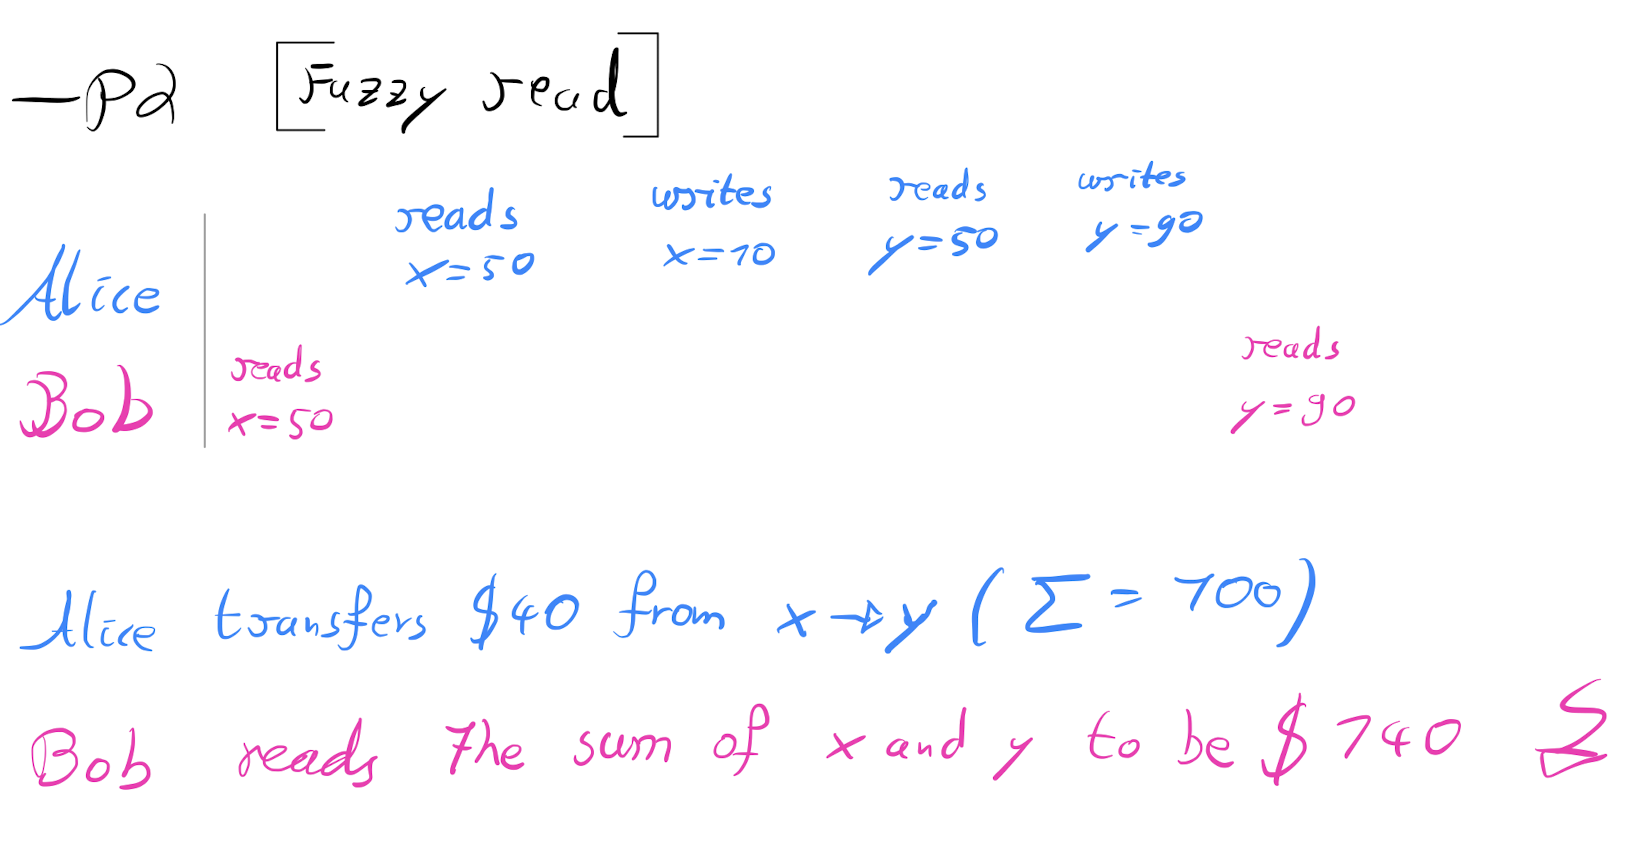
\includegraphics[width=8.5cm]{P2}
    \caption{History for P2}
    \Description{P2}
\end{figure}

\begin{example}
    Bob starts to read the sum by reading x and gets interrupted by Alice who transfers 40€ from account x to y.
    After this is completed Bob reads the value of y.
    Thus the sum is 100€ for Alice while it is 140€ for Bob.
    In contrast to \textbf{P1} a second read of x by Bob would have returned the correct sum of 100€.
\end{example}
\subsection{P3 - Phantom}
Once again when looking at the ANSI specification one can see that it only disallows inserts on the \emph{serializable}
isolation level while the following definition of \textbf{P3} prohibits deletions, inserts, and updates, making it stronger than \textbf{A3}.
This phenomenon is only applicable to transactions using predicates and applies to deletions, insets, and updates.

\begin{figure}[h]
    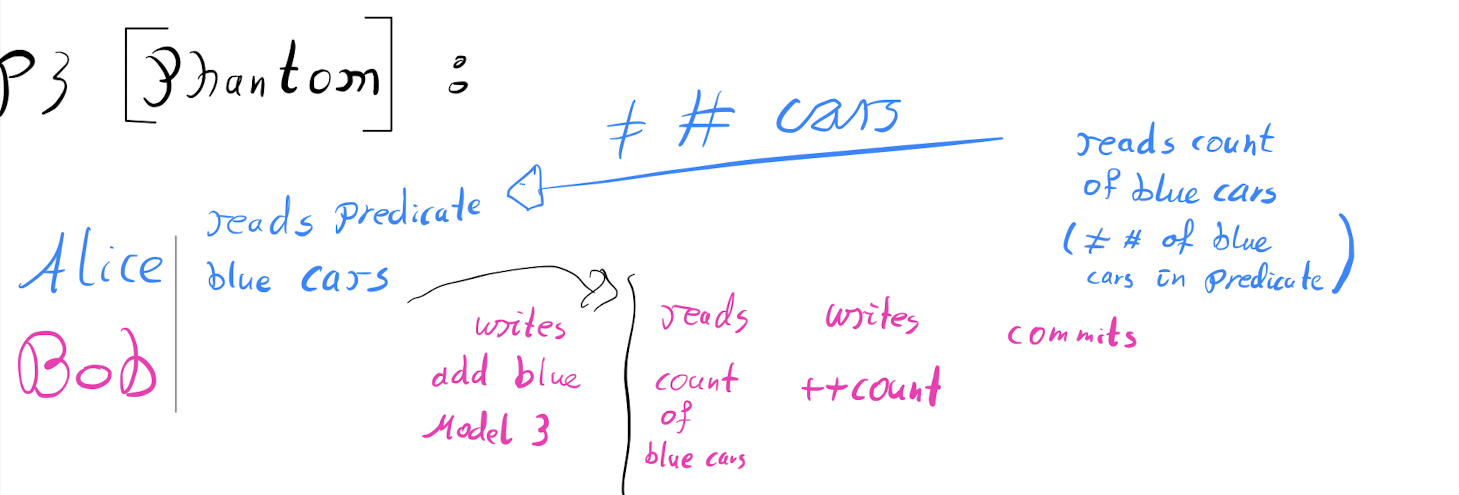
\includegraphics[width=8.5cm]{P3}
    \caption{History for P3}
    \Description{P3}
\end{figure}

\begin{example}
    Alice reads the predicate blue cars. Bob then adds a new blue car to the database and increases
    the count of blue cars. Alice then reads the count of blue cars. This leads to a phantom item
    (Alice can’t see Bob's car but knows of its existence due to the increased count).
\end{example}
Not prohibiting this phenomenon can cause inconsistent predicate reads and in the worst case phantom entries in the
database as the reading transaction could, after reading a phantom object, either assume that it does not exist or treat it like an actual
object,. Both situations would lead to undefined behavior of the transaction.

\section{ANSI isolation levels}
We define the isolation levels by the phenomena prohibited by it and we define
Degree 0 isolation to be the isolation level that does not prohibit any abnormal
behavior. Furthermore, we define short duration locks as locks that are held
while a transaction reads or writes an item, in contrast to long-duration locks which are
held until a transaction commits or aborts.
These definition can then be used to classify different database system implementations in
regards to their serializability.

\subsection{Read uncommitted}
We define \emph{read uncommitted} to be the isolation level that prohibits the phenomenon
P0, \emph{dirty write}. This can be accomplished by placing \emph{long-duration write locks} when modifying a data item.
This only allows one transaction at a time to write to a given value and requires all others to wait for a commit or abort.

\subsection{Read committed}
Read committed is defined as the isolation level where \textbf{P1}, \emph{dirty read} is prohibited.
To accomplish this the use of \emph{short duration read locks}, as well as \emph{long write locks}, is
necessary. Thus disallowing a write on an data item that was just read by another transaction, as
well as disallowing overwriting of an item already written by another, unfinished, transaction.

\subsection{Repeatable read}
For \emph{repeatable read}, the phenomenon \textbf{P2}, \emph{fuzzy read}, has to be prohibited.
This requires \emph{long duration write locks} as well as \emph{long duration read locks} on
items and \emph{short duration locks} on predicates.\\
The difference to \emph{read committed} is that in the \emph{read committed} isolation level it is only guaranteed that
the data read was committed at the time of reading (no dirty reads). Whereas
\emph{repeatable read} also guarantees that the data read will not change before the
transaction finishes either with a commit or abort.

\subsection{Serializable}
For serializability the phenomenon \textbf{P3} needs to be prohibited, which can be done by placing \emph{long locks
    on reads and writes}. This isolation level is stronger then it's ANSI counter part due to the
prohibition of predicate updates and deletions as defined in \textbf{P3}, making it the only isolation level
stronger than the original ANSI serializable isolation level specification.

\section{Cursor stability}
For the isolation level \emph{cursor stability}, it is useful to define a fourth phenomenon \textbf{P4} (\emph{lost update}), as this isolation level
was designed to solve the problem of lost updates.
\subsection{ P4 - lost update}
This phenomenon describes the loss of an update to an data item by a transaction, due to it immediately being overwritten
by a second transaction.

\begin{figure}[h]
    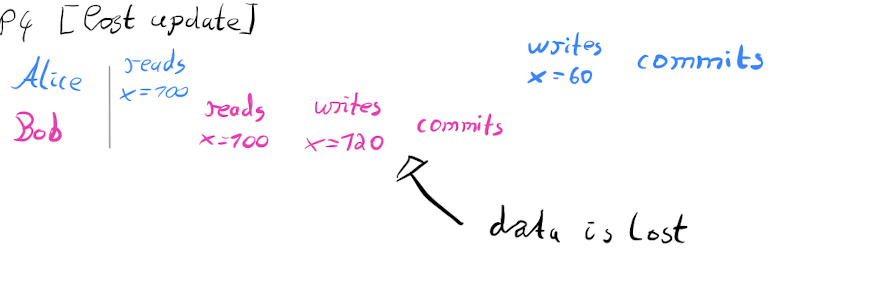
\includegraphics[width=8.5cm]{P4}
    \caption{History for P4}
    \Description{P4}
\end{figure}

\begin{example}
    Alice reads x to be 100€. Bob then reads the same, adds 20€ and writes 120€ to x and commits.
    Alice then subtracts 40€ from x and writes 60€ to x and commits, resulting in the loss of Bob's update.
\end{example}

\subsection{Implications}
The phenomena define above can be prohibited by placing a read lock on x (position of the cursor) when
read and placing a long write lock on the items row when modified.
The read lock is removed when the cursor moves (e.g. reading a new tuple),
while the write lock only gets removed after the transaction commits or aborts.\\
As \emph{Cursor stability} is stronger then \emph{read committed} while being weaker then \emph{repeatable read}, it
is used instead of the weaker \emph{repeatable read} by some database systems. This behavior is allowed by the ANSI standard
as it defines a minimum set of guarantees.
\subsection{Strength}
When looking at the isolation levels defined in section 2, one can see that \textbf{P4} is prohibited by \emph{repeatable read},
as \emph{long duration locks} on reads and writes will also disallow the overwriting of an item by another transaction.
\emph{cursor Stability} is thus weaker than \emph{repeatable read} as prohibiting \textbf{P4} does not prohibit \textbf{P3}.
Looking at \emph{read committed}, one can reason that a transaction A can read x, then be interrupted by transaction B which updates
item x and commits, and transaction A then continues to write to x.
Thus making \emph{Cursor stability} stronger than the strengthened \emph{read committed}.
\subsection{Multi cursor}
While the \emph{Cursor stability} based system described above could also be extended with the use of multiple cursors, thus
parleying the effect of \emph{repeatable read} isolation, as long as each transaction does not access more items
then the system has cursors. But obviously this is neither a general, nor even a practical solution to the phenomenon \textbf{P2} and
although it might have real life use cases it will not be discussed further in this paper.
\section{Snapshot Isolation}
While all of the above-mentioned systems suggest lock-based implementations, this is not the only way to prohibit the defined phenomena.
In contrast we will look at
\emph{snapshot isolation} which uses multi-versioning to prohibit these phenomena.\\
In \emph{snapshot isolation}, each transaction gets it's own snapshot of all committed data at it's start,
thus reads are never blocked. All writes are performed on the given snapshot as to not disturb
other transactions. Reads of the updated data is only allowed for the same transaction that wrote them (unless the transaction has committed).
For the committing procedure, a second (commit) timestamp is assigned, said timestamp is larger than every
other assigned time stamp in the system. If another transaction A already modified data of the committing
transaction B it's commit fails, leading to an abort.
\subsection{P5B - Write skew}
To take a closer look at the difference to \emph{repeatable read} it is useful to define a new phenomenon.

\begin{figure}[h]
    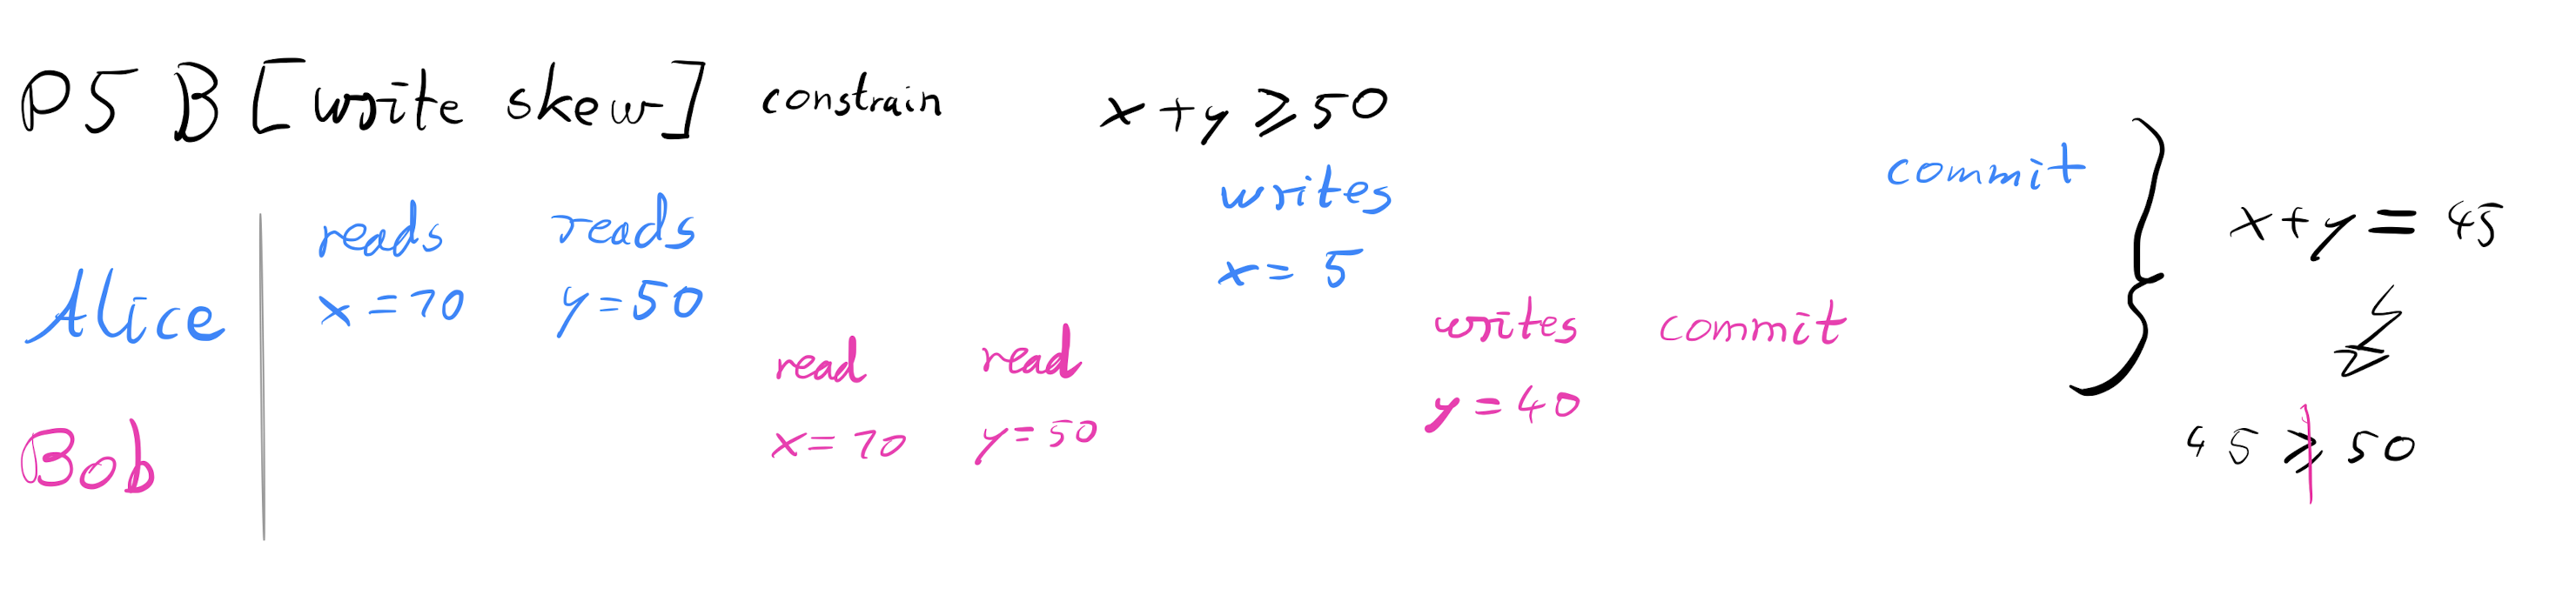
\includegraphics[width=8.5cm]{P5}
    \caption{History for P5}
    \Description{P5}
\end{figure}

\begin{example}
    (assuming first commit wins):
    Constraint: $ x+y \geq  50$
    Alice reads x to be 10€ and y to be 50€. Bob then reads the same data, while getting his own snapshot
    to operate on (newer timestamp than Alice). Alice then sets x to be 5€,
    resulting in a sum of 55€. Bob then sets y to be 40€. Alice commits and Bob then commits resulting in a sum of 45€.
\end{example}

\subsection{Implications}
When looking at the phenomena defined above one can see that prohibiting it with a locked based system
would be equal to prohibiting \textbf{P3} as a lost update can only be prohibited by placing long locks on all reads and writes.
But when using a multi version system instead, proscribing \textbf{ \textbf{P5B}} is not equal to proscribing \textbf{P3}.\\
The example in subsection 5.1 is allowed by \emph{Snapshot isolation} as it does not check for constrains and the transactions
does not modify the same item (x and y respectively). \emph{Repeatable read} on the other hand would disallow such
behavior as it places \emph{long read} and \emph{write locks} on the items.\\
\textbf{P5B} is thus useful to differentiate between \emph{Snapshot isolation} and \emph{repeatable read}.
\subsection{Comparison with repeatable read}
As stated above \emph{repeatable read} prohibits \textbf{P5B} while \emph{snapshot isolation} prohibits some cases of
\textbf{P3} and both prohibit \textbf{P0}, \textbf{P1}, and \textbf{P2}. Although the argument above is made with a locking implementation
it is general as the phenomena defined were strengthened to match the behavior of locking implementations. \\
\emph{Snapshot isolation} is comparable in strength to \emph{repeatable read} as both prohibit \textbf{P0}, \textbf{P1}, and \textbf{P2}.
To further investigate their difference we have to take a look at the original ANSI specification of \emph{serializable},
as it prohibits	\textbf{A3}, which will be defined in the following section.
\subsection{A3 - Anomaly Phantom}
This is the strict interpretation of the Phantom anomaly. The difference to \textbf{P3} is that the position of the
transactions commit is not indifferent for \textbf{A3}.
\begin{example}
    Alice reads the predicate blue cars. Bob then adds a new blue car to the database and increases
    the count of blue cars. Bob commits.  Alice then reads the count of blue cars. This leads to a phantom item
    (Alice can’t see Bob's car but knows of its existence due to the increased count).
\end{example}
Thus \textbf{A3} only operates on committed data while \textbf{P3} also accounts for transactions to still be in progress,
making \textbf{A3} a weaker phenomenon than \textbf{P3}.
\subsection{Comparison to ANSI}
When looking at the weak interpretation of the ANSI specification as in \cite{Adya_Liskov_O_Neil_2000}
one can see that Snapshot isolation prohibits all three anomalies \textbf{P1}, \textbf{P2}, and \textbf{A3} making it \emph{anomaly \emph{serializable}}.
To show this we will now take a look at \textbf{A3} as we have already shown above that Snapshot isolation prohibits \textbf{P1} and \textbf{P2}.
As the definition of \textbf{A3} states the importance of commit sequence it is easy to see that Snapshot isolation with a first commit wins
strategy precludes \textbf{A3}, as a already altered item will lead to an abort of the transaction that tries to commit.
When looking at a first write wins the same is true as still only one modified value will
be written to the database and the other one will be discarded by an abort. It thus only changes
which transaction wins in comparison to first commit wins.
\subsection{Comparison to Serializable}
In comparison to the \emph{serializable} isolation level defined in section 3.4 we can say that Snapshot isolation is
weaker as \emph{serializable} precludes \textbf{P5B} as well as \textbf{P3}, which as shown in example 5.1 above does not hold true
for Snapshot isolation.
\section{Conclusion}

In conclusion one can see that the ANSI SQL specification is inherently flawed when talking
about multi-version histories and other non locking database systems, as it failed to consider
these systems when defining the phenomena. This will inevitably lead to different interpretations
and implementations. To ensure the correct behavior of non locking implementations of ANSI SQL it might be advisable to update the ANSI standard
according to the definitions discussed above and in \cite{Adya_Liskov_O_Neil_2000} and \cite{Berenson_Bernstein_Gray_Melton_O_Neil_O_Neil_1995}.
\bibliographystyle{plainnat}
\bibliography{refs}

\end{document}